\documentclass[letterpaper, 10 pt, conference]{ieeeconf}
\IEEEoverridecommandlockouts
\overrideIEEEmargins{}
% Language
\usepackage[english]{babel}
% Graphics
\usepackage[pdftex]{graphicx}
\usepackage{adjustbox}
\graphicspath{{./figures/}}
\DeclareGraphicsExtensions{.pdf,.jpg,.jpeg,.png}
% Math
\usepackage[cmex10]{amsmath}
\interdisplaylinepenalty=2500{}
% Floats
\usepackage{booktabs,multirow}
\usepackage[caption=false,font=footnotesize]{subfig}
% URLs
\usepackage{url}
% Useful Macros
\newcommand{\fref}[1]{Fig.~\ref{#1}}
\newcommand{\tref}[1]{Table~\ref{#1}}
\newcommand{\sref}[1]{Section~\ref{#1}}
\newcommand{\code}[1]{\texttt{#1}}
\newcommand\mat[1]{\boldsymbol{#1}}
\newcommand\vect[1]{\boldsymbol{#1}}
\newcommand\matop[2]{\boldsymbol{#1}\left({#2}\right)}

\title{\LARGE \bf{}
Contact Force Estimation for Robotic Assembly using Motor Currents/Torques
}

\author{Raymond Djajalaksana, Francisco Suarez, and Quang-Cuong Pham}

\begin{document}
\maketitle
\pagestyle{plain}
\thispagestyle{plain}

% Content
\begin{abstract}
In robotic assembly task, the robotic arm must be able to cooperate with a lot of uncertainites in the dynamic environment. Thus, the ability to know about contact force is crucial in assembly robot. This paper studies about the identification of all parameters required to measure contact force via motor currents. The study also includes two friction models to be identified and how well it is to estimate the contact force. The results are obtained and presented in this paper. 


\end{abstract}

      \section{Introduction}
In robotic assembly task, the robotic arm must be able to cooperate with a lot of uncertainites in the dynamic environment. For example, the manipulator has to be able to know when the contact with an object is happening. This ability requires knowledge of contact force for the robot. Thus, estimation of contact forces is very crucial since it will help the robot to determine the contact with objects in dynamics environment. While this can be done using accurate force/torque sensor, the sensor is normally expensive and requires mechanical integration with the robotic arm \cite{Hao15}. Thus in some arms it might not be possible to attach this sensor.   

In regards to this, many researches have been done in order to estimate the contact force. The main idea to estimate the contact force is to directly apply dynamic equations of a robot, knowing the value of joint torques. However different approaches have also been explored in the past few decades. Early approaches use observers for force estimation like in \cite{Ohi91}. Another approach in \cite{Stolt12} involves detune the low-level joint position control loop to estimate contact force. Furthermore, recent approaches by using Bayesian approach and generalized momentum with Kalman filter are studied in \cite{Hao14} and \cite{Hao15} respectively. Additionally, a study of comparison between two different approaches are done in \cite{Beyl11}. The study compares the result from filtered dynamic equation of external force with generalized momentum method.

This paper aims to estimate contact force based on motor currents and finally develop the algorithm to control the contact force of the robot. The model for the force estimation is still based on the basic dynamic equation. 

%----------------------------------------------------------------------------------------------------

      \section{Model Estimation}
The basic dynamic equation of robotic arm is described by:
\begin{align}
  \tau_{mot} &= \tau_{dyn} + \tau_{ext} + \tau_{friction}\\
  \tau_{dyn} &= H\left(q\right)\ddot{q} + C\left(\dot{q} , q \right)\dot{q} + G\left(q \right)\\
  \tau_{ext} &= J^{T} F_{ext}\\
  \tau_{mot} &= K_{m} I_{mot}
\end{align}

The aim is to get the value of the $K_{m}$ parameter and $\tau_{friction}$ having known other values. The value of $\tau_{dyn}$ is estimated from computer using OpenRave.

The friction here can be described further with various model. In this paper two kind of friction models are considered. The first one is a simple static friction which use coulomb and viscous friction model. Using coulomb and viscous model, the friction can be modeled as:

\begin{equation}
  \tau_{friction} = K_{c} sign\left(\dot{q}\right) + K_{v} \dot{q}
\end{equation}

And the second one is by using Dahl model which is a basic dynamic friction. Dahl mathematical model relies on some internal state that can explain the lag of change because of friction \cite{Bona05}. This model should picture more realistic than coulomb and viscous model. The basic equation is: 

\begin{align}
  \dot{z} &= \dot{q} - \frac{\left|\dot{q}\right|}{F_{c}} \sigma z \\
  \tau_{friction} &= \sigma z
\end{align}

The result of friction identification is presented in the \ref{identification}.

%----------------------------------------------------------------------------------------------------

      \section{Experimental Setup}
The manipulator arm that was used is Denso VS060A3. Motor currents and torques were available from Denso and ATI Gamma F/T sensor was attached at the end-effector arm to get the contact force value.  
   
\subsection{Setup}
\label{setup}
The procedures to get data for first, second, third, and fifth joint are similiar while fourth and sixth joint followed different procedure. the difference happened simply because of the feasibility of performing the experiment, thus there is no specific reason for it. The first type of experiment is described as follow. First the arm moved to a pre-contact position near a fixed object or ground (\fref{fig:setup 1 precon}). Thereafter the arm moved slowly approaching the object until the F/T sensor got a reading above 1 N. When the contact had been made (\fref{fig:setup 1 con}), the robot will push the object/ground in a sinusoidal motion.

On the other hand, the setup for fourth and sixth joints are like this (\fref{fig:setup 2}): The arm will move to a fixed position and it would remain static thereafter. While the robot remained static, external forces and/or torques were introduced using hand. These forces/torques were applied in such a way that the fourth and sixth joint would be the most affected one.

Motor currents, joint positions, and external force/torque were recorded during all the experiment.

\begin{figure*}[ht]
  \centering
  \subfloat[First setup (Pre-contact)]{
    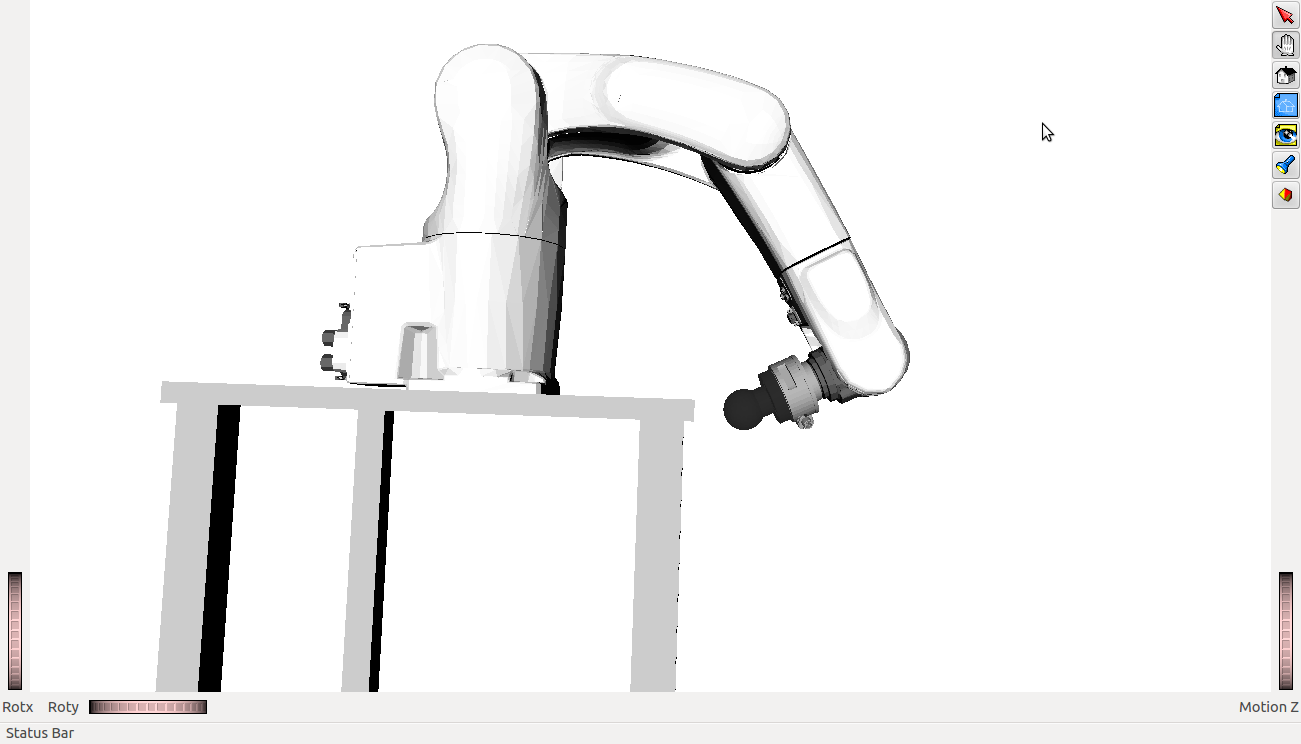
\includegraphics[width = 0.3\textwidth ]{fig01} 
    \label{fig:setup 1 precon}}\,
  \subfloat[First setup (Contact)]{
    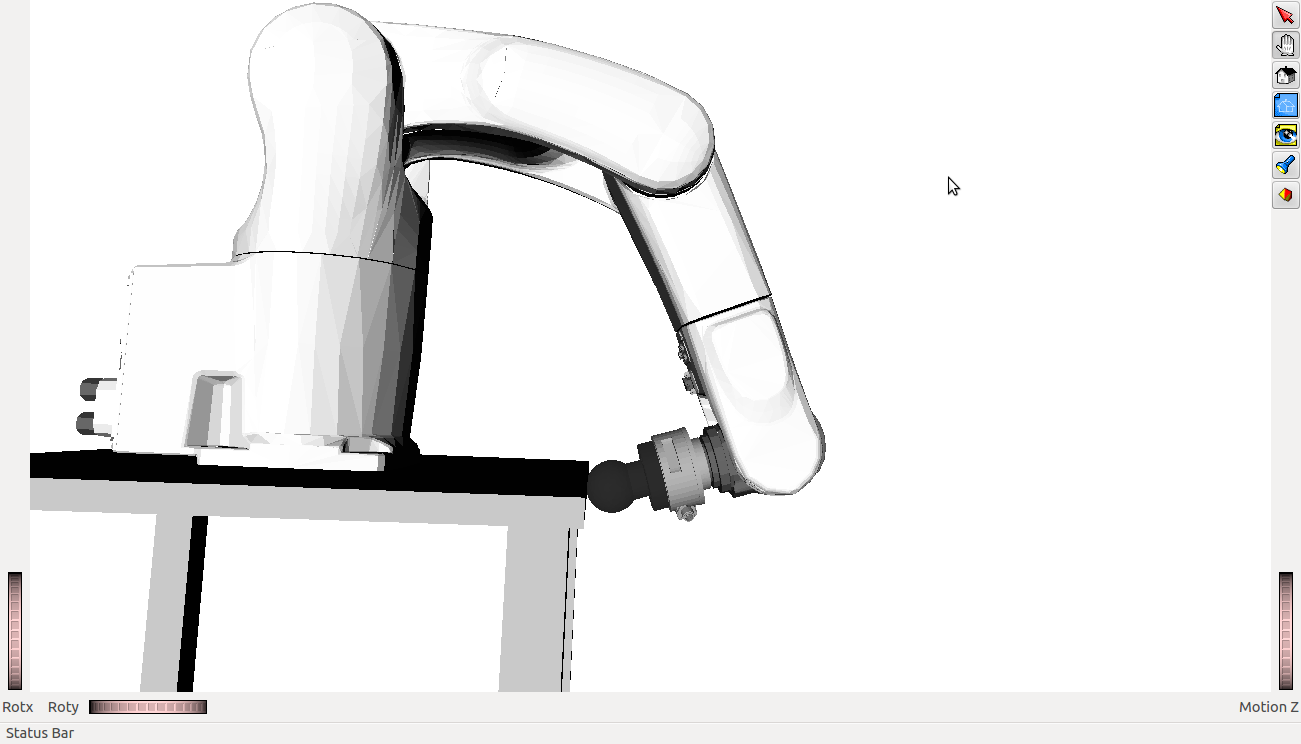
\includegraphics[width = 0.3\textwidth ]{fig02} 
    \label{fig:setup 1 con}}\,
  \subfloat[Second setup]{
    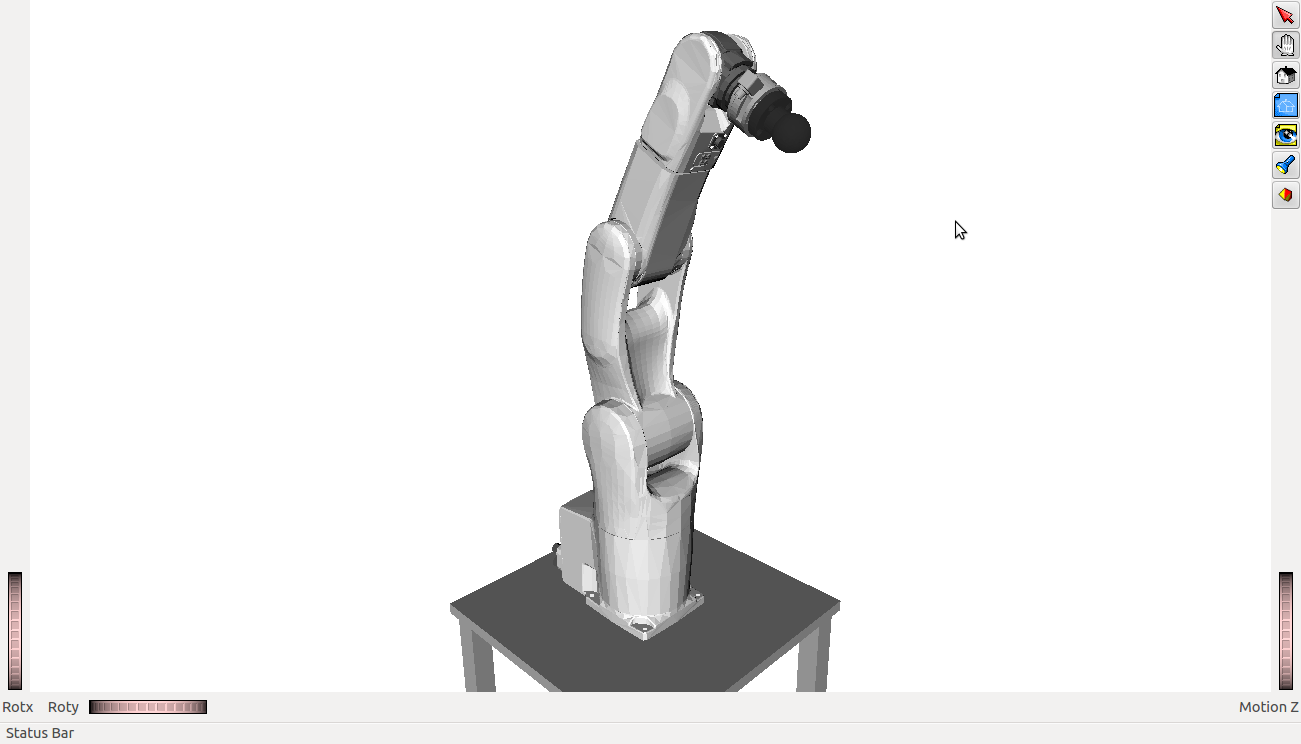
\includegraphics[width = 0.3\textwidth ]{fig03}
    \label{fig:setup 2}}\,
  \caption{Setup of experiments}
\end{figure*}

\subsection{Motor Currents Reading}
Before continue with more experiment and identification, there is one problem that needs to be solved first. The problem is that the arm only gives absolute value of the motor currents (\fref{fig:raw current}). Thus there is a need to identify the sign of the motor currents of each joints. Three methods were tried but only one was successful.

The first attempt was to give the motor current sign based on the sign of $\tau_{dyn}$ during non-contact condition. However, this poses a problem when the $\tau_{dyn}$ goes near zero as it will not be clear enough to identify the sign. The second method was to match the derivative of motor currents with derivative $\tau_{dyn}$ during pre-contact motion (e.g.: if $\tau_{dyn}$ is increasing, the motor currents has to be increasing too, and vice versa). Unfortunately, this principle working only if motor currents are very smooth and steady which is a very difficult condition.

After the first two attempts, it was found out that we can actually extract motor torques value from Denso and this time it includes the sign of it. While the value cannot be used directly to the equation since there is too few information about the value, the sign of torques can be used to determine the sign of motor currents. With this, now we can know the real motor currents of each joints (\fref{fig:mod current}).

\begin{figure}
  \centering
  \subfloat[Raw motor currents]{
    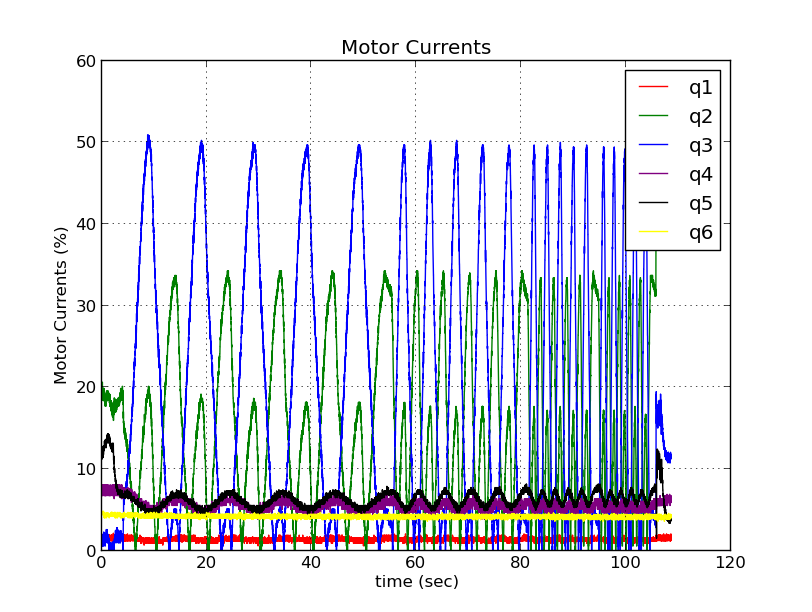
\includegraphics[width = 0.45\textwidth ]{fig04} 
    \label{fig:raw current}}\,
  \subfloat[Motor currents using sign of motor torques]{
    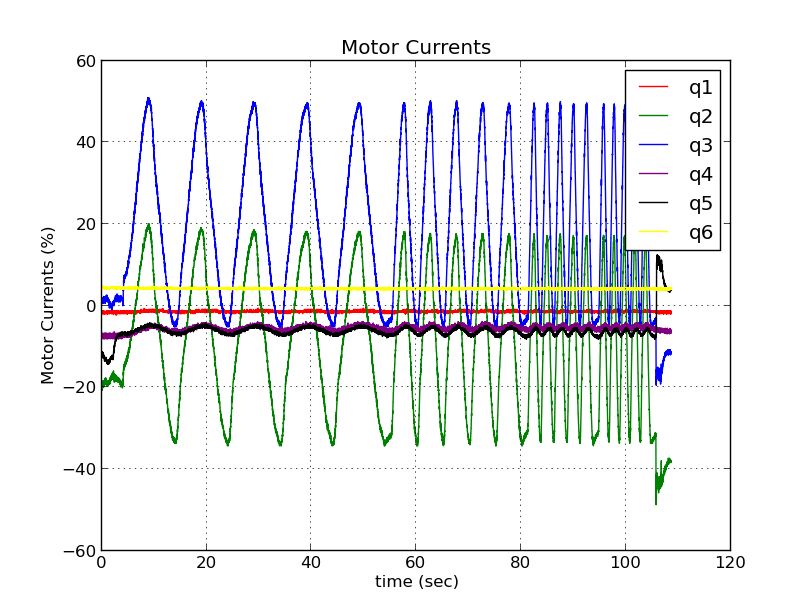
\includegraphics[width = 0.45\textwidth ]{fig05}
    \label{fig:mod current}}\,
  \caption{Reading of motor currents}
\end{figure}

%----------------------------------------------------------------------------------------------------

      \section{Results}
\subsection{Preliminary Results}
The result of experiments can be seen in \fref{fig:prelim result}. The reference value (zero-value) of both axis is the value of pre-contact position. It shows quite a different results for fourth and sixth joint with any other joints result. This is due to the experimental setup for these two joints are different as it has been explained in \ref{setup}.

\begin{figure*}[t]
  \centering
  \subfloat[First Joint]{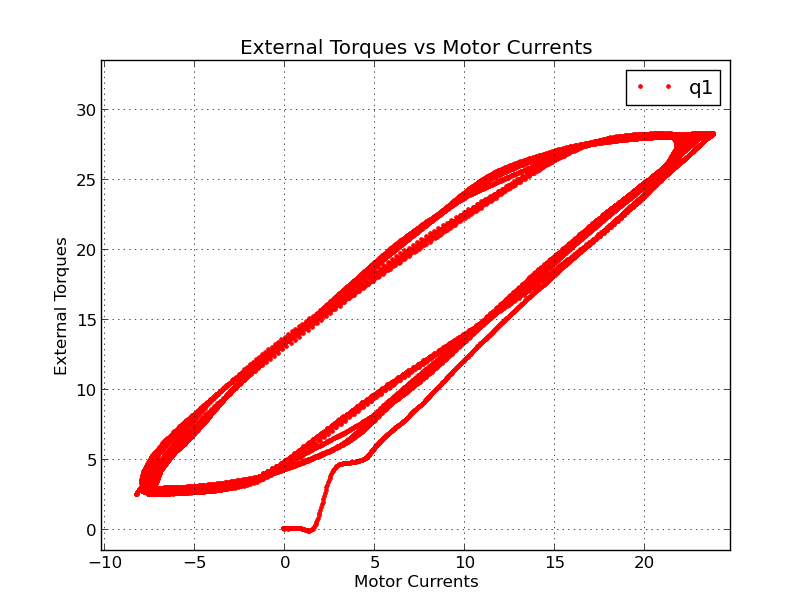
\includegraphics[width = 0.3\textwidth ]{fig06}} \,
  \subfloat[Second Joint]{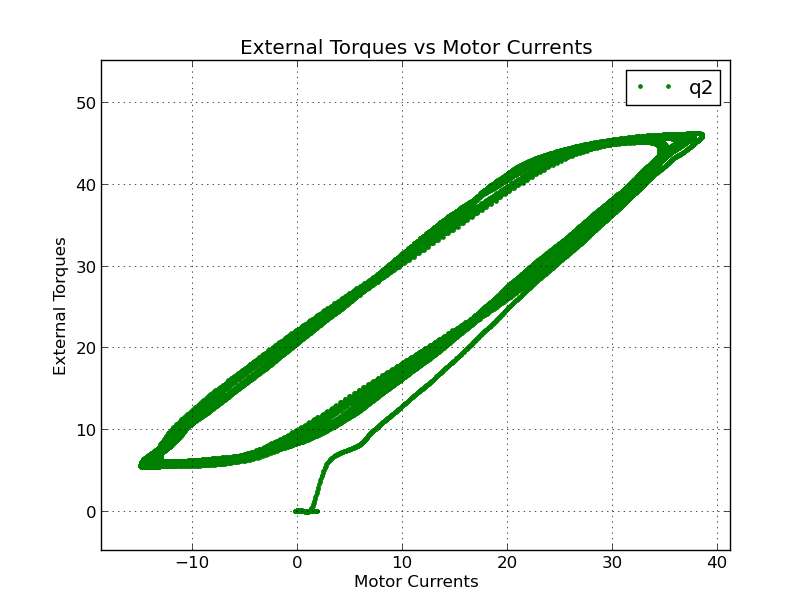
\includegraphics[width = 0.3\textwidth ]{fig07}} \,
  \subfloat[Thrid Joint]{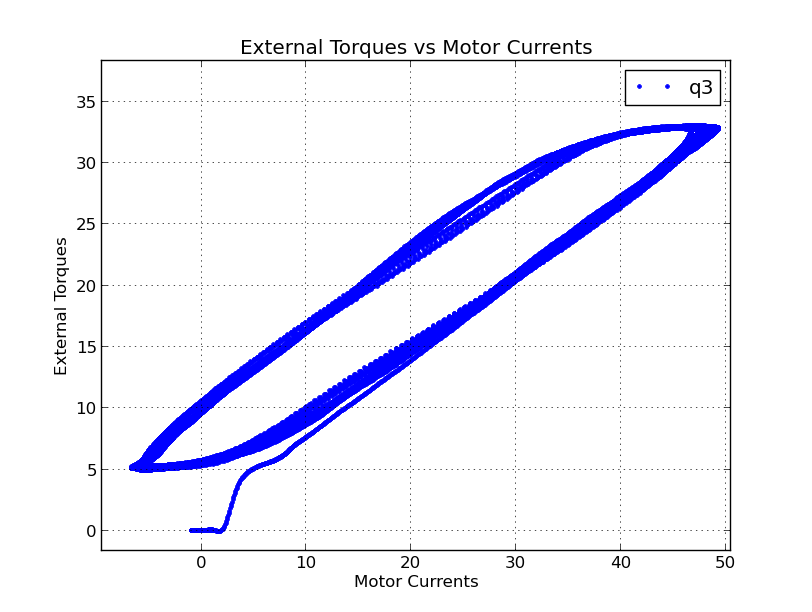
\includegraphics[width = 0.3\textwidth ]{fig08}} \,
  \subfloat[Fourth Joint]{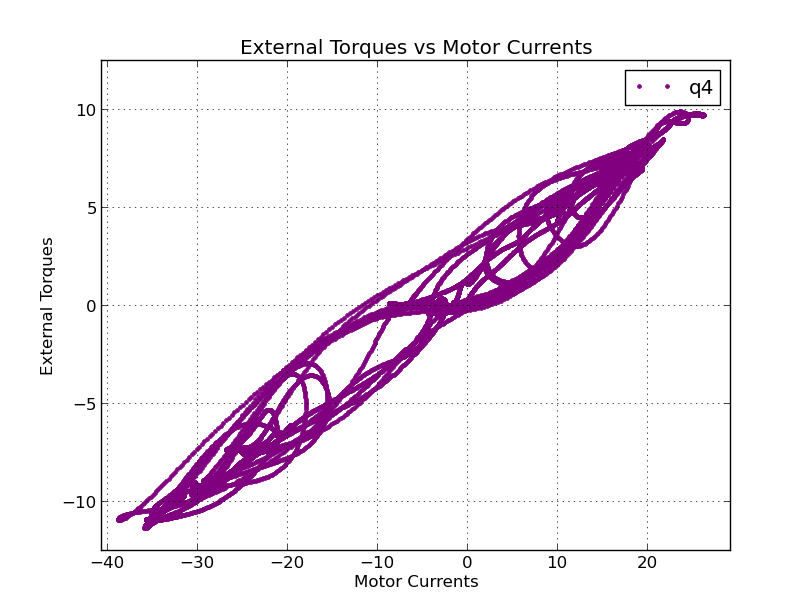
\includegraphics[width = 0.3\textwidth ]{fig09}} \,
  \subfloat[Fifth Joint]{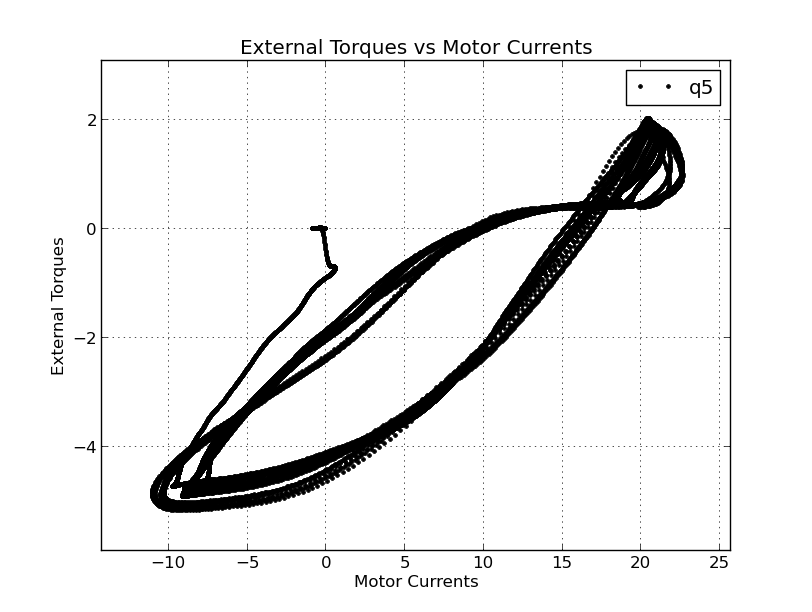
\includegraphics[width = 0.3\textwidth ]{fig10}} \,
  \subfloat[Sixth Joint]{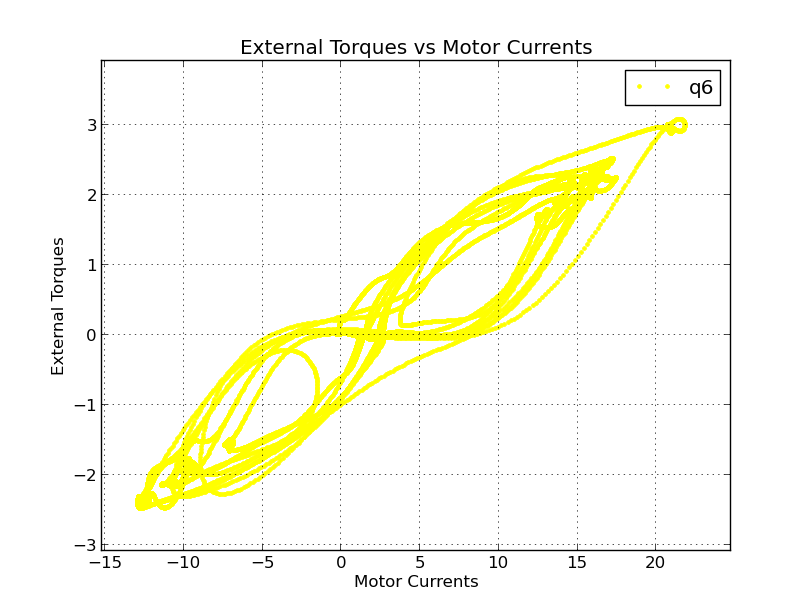
\includegraphics[width = 0.3\textwidth ]{fig11}} \,
  \caption{ External torques vs motor currents}
  \label{fig:prelim result}
\end{figure*}

\subsection{Model Identification}
\label{identification}

Firstly, the value for identification is referenced with pre-contact condition. From computation it is known that there is only a few changes in $\tau_{dyn}$ during contact motion and so it can be ommitted. Thus, the dynamic equation can be simplified into just:

\begin{equation}
  J^{T} \Delta F_{ext} = K_{m} sign\left(\tau_{mot}\right) \Delta I_{mot} - \Delta \tau_{friction} + C
\end{equation}
 
Here we introduces a constant to adjust for any offset thay may happen. As for friction, we will identify it using static friction and Dahl friction. As for Dahl friction, some adjustments to the equation need to be done to match with the optimization. The modified Dahl equation that is going to be used is : 

\begin{align}
  \dot{z} &= p_{2 }\dot{\tau_{mot}} - \left|\dot{\tau_{mot}}\right| p_{3} z \\
  \tau_{friction} &= p_{1} z
\end{align}

To identify all the unknown parameters, the equation is optimized to match with the fitted data. The number of parameters to be optimized will depend on the model of friction that we choose. This optimization is done by using nelder-mead method. One of the result of optimization is shown in \fref{fig:optimization}. It shows the result for both friction model that is going to be used. 

From \fref{fig:optimization}, it is quite clear that result will depend on the friction model that we choose. Using Dahl model, the error value to the fitted data is less than using coulomb + viscous friction. However, Dahl model imposes one problem. The model requires initial state of $z$. During optimization, this value is unknown and hence it was optimized together with other parameters. However, this initial state will always change for every different position of the arm. Thus, it makes the model more difficult to implement since we need to know the initial state. This will be more clear in the next subsection (\ref{validation}).

\begin{figure}
  \centering
  \subfloat[Using viscous and coulomb model]{
    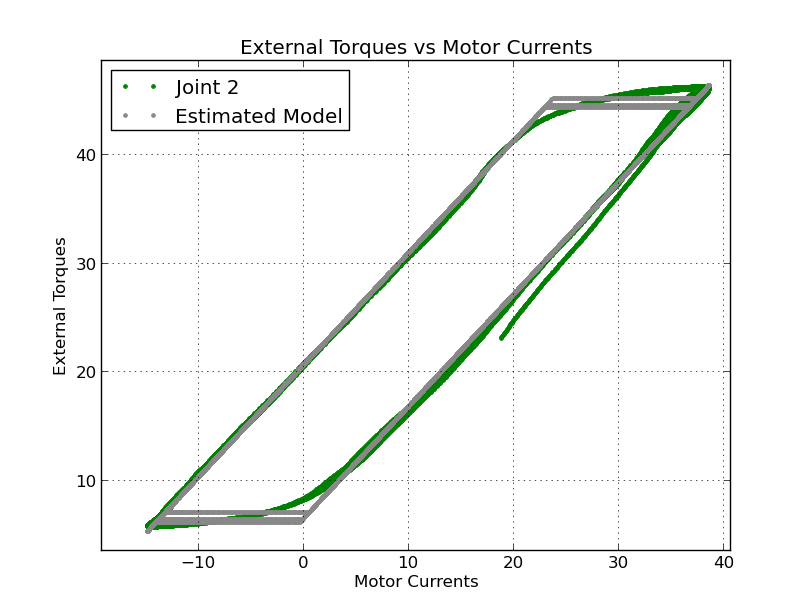
\includegraphics[width = 0.45\textwidth ]{fig12} 
    \label{fig:raw currents}}\,
  \subfloat[Using Dahl model]{
    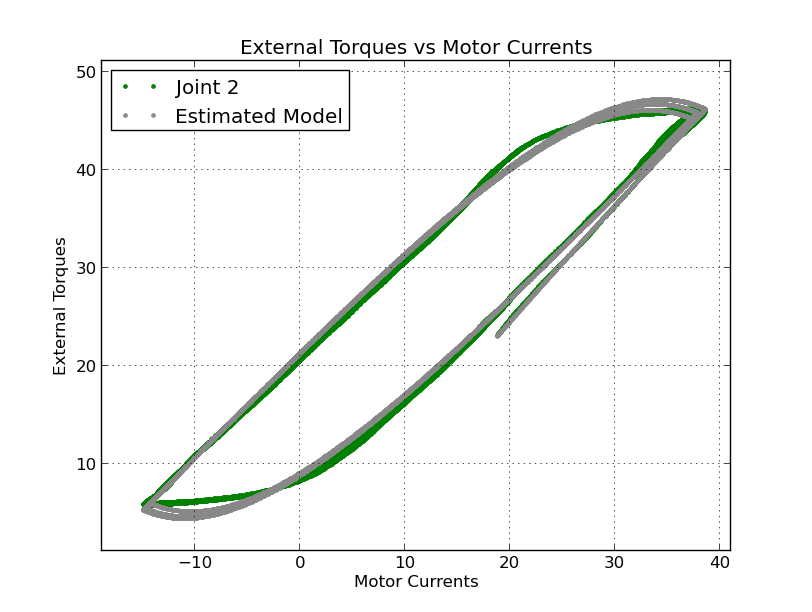
\includegraphics[width = 0.45\textwidth ]{fig13}
    \label{fig:mod currenta}}\,
  \caption{Example of optimization result of one joint (e.g.:second joint)}
  \label{fig:optimization}
\end{figure}

\subsection{Validation}
\label{validation}

After identifying the paramaters for all the required equation, developed algorithm model now was built to estimate the contact force. Hence, there are two versions of algortithm, one that use Dahl and another one that use coulomb and viscous. The estimated force is then compared to real force from F/T sensor for validation. The results are shown in \fref{fig:validation} 

In \fref{fig:Dahl tor} it is quite clear that Dahl algorithm gives a good estimation for second and third joint. However, it is bad when estimating the first joint. This is more likely due to two reasons. First, the initial state of $z$ might be incorrect. For every arm position, it is supposed to have specific state of $z$, however as we lack of knowledge of this value, it was only calculated using some basic assumption. The second reason is due to stability of motor currents. Since change of internal state is a function of rate of motor currents, unstable motor currents will drift the value of $z$. However, seeing that the value of first joint seems drifted over time, hence it is more likely that the second reason is the main problem.

On the other hand, the results using coulomb and viscous can be seen in \fref{fig:static validation} and \fref{fig:static tor}. The estimated force in x-axis is quite satisfactory and this is the main force that acting on the robot. However, the force estimation of other axis is not as good as the first one. This is because of the error estimation of external joint torques that leads to the force. The comparison of external joint torques estimation can be seen in \fref{fig:torque validation}. The root mean square error values of estimated contact force and torque using this model are presented in \tref{table:rmse}.

\begin{table}
    \centering
    \begin{tabular}{| c | c | c | c |}
    \hline
              & RMSE & max-min & RMSE / (max-min)(\%) \\ \hline
    Force x   & 5.231976  & 107.774842  & 4.854543  \\ \hline
    Force y   & 0.942644  & 2.391211    & 39.421205  \\ \hline
    Force z   & 18.686503 & 32.631091   & 57.265945  \\ \hline
    Torque x  & 0.116993  & 0.048434    & 241.550320  \\ \hline
    Torque y  & 3.542738  & 0.879940    & 402.611434  \\ \hline
    Torque z  & 0.350672  & 0.192694    & 181.983440  \\ \hline
    \end{tabular}
    \caption{Root mean square value of estimated contact force using static friction}
    \label{table:rmse}
\end{table}

One point to be considered is that since the algorithm model for static friction has some discrete characterics, it will have two effects on the estimation. First, the estimated contact force will have discrete pattern, which might be undesirable if certain cases need continuous profile. Second, The value will not change unless it overcomes the threshold of discrete value. This might be bad if the changes in the input (motor currents in this case) is small, since it will not counted as a change. However, these two effects do not happen in Dahl model since it is a continuous equation.  

Hence, based on validation results both of friction model have their own advantages and disadvantages. For this reason, both models will be kept for further testing of controlling the robot. 

\begin{figure}
  \centering
  \subfloat[Validation using viscous and coulomb friction]{
    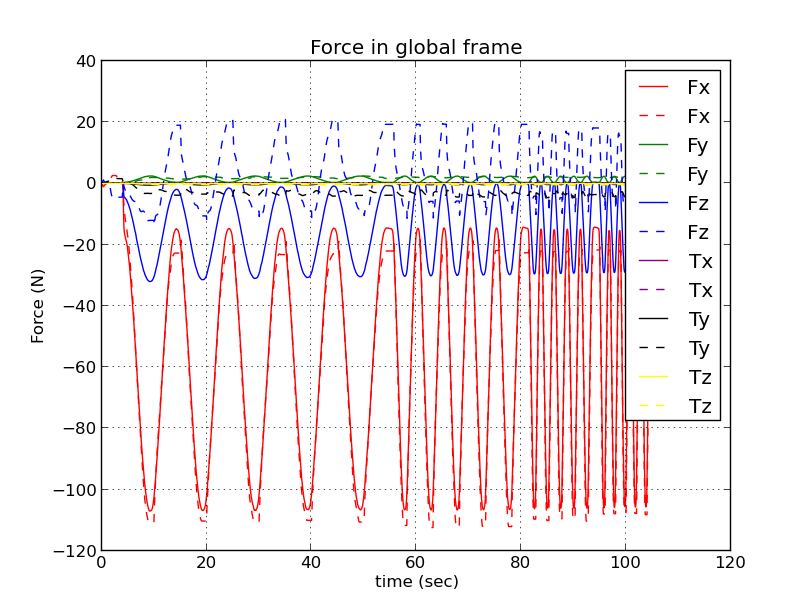
\includegraphics[width = 0.35\textwidth ]{fig14} 
    \label{fig:static validation}}\,
  \subfloat[Validation using Dahl model]{
    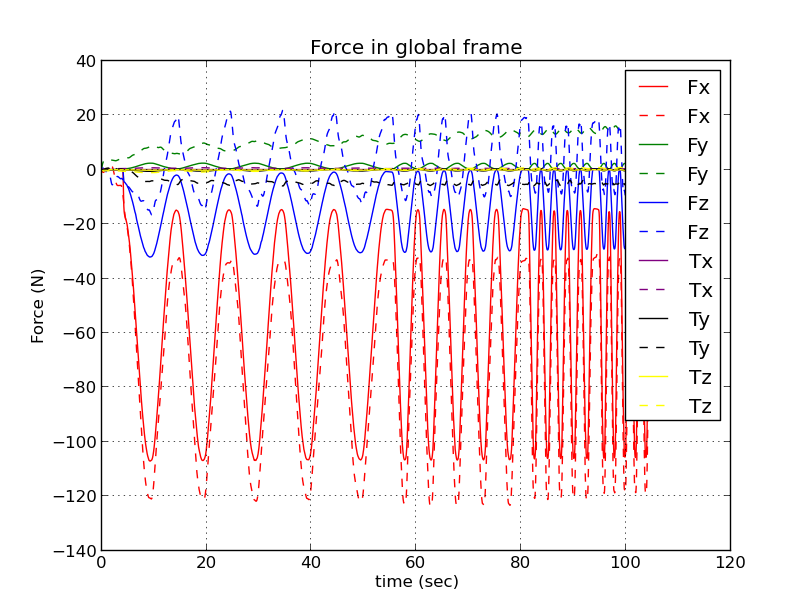
\includegraphics[width = 0.35\textwidth ]{fig15}
    \label{fig:Dahl Validation}}\,
  \caption{Validation result of estimated force. (- - : estimated output, -- : real output)}
  \label{fig:validation}
\end{figure}

\begin{figure}
  \centering
  \subfloat[Using static model]{
    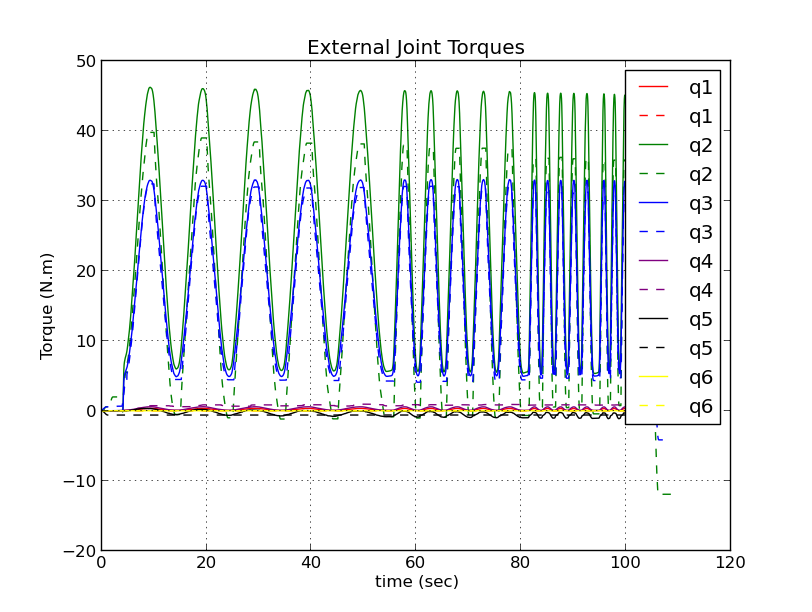
\includegraphics[width = 0.35\textwidth ]{fig16} 
    \label{fig:static tor}}\,
  \subfloat[Using Dahl model]{
    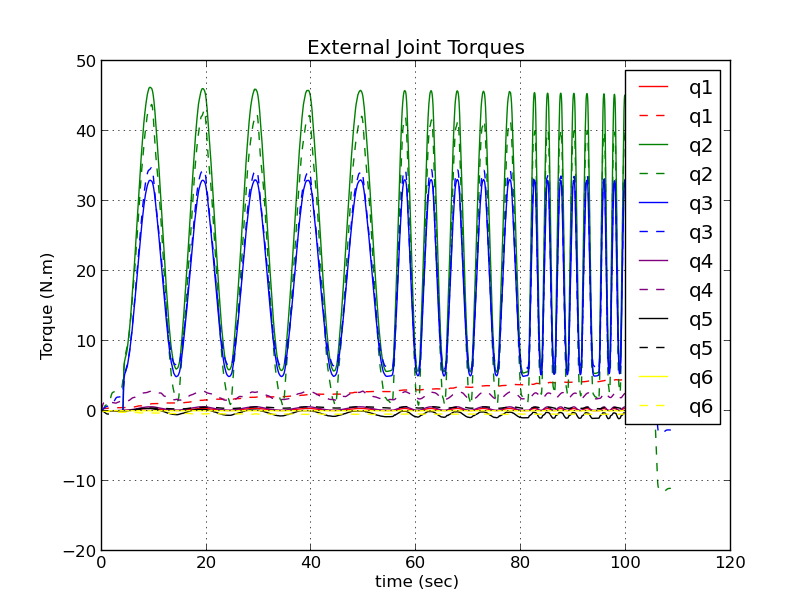
\includegraphics[width = 0.35\textwidth ]{fig17}
    \label{fig:Dahl tor}}\,
  \caption{External joint torques estimation of \fref{fig:static validation} (- - : estimated output, -- : real output)}
  \label{fig:torque validation}
\end{figure}

%----------------------------------------------------------------------------------------------------

      \section{Future Works}
Future works include testing the identification results and the developed algorithm for both friction in real time operation. After that, we can finally start to control the robot to perform assembly task (e.g.: pin insertion) with the tested results. Finally, we will compare the result of both model and choose the best one.

%----------------------------------------------------------------------------------------------------

      \section{Conclusion}
Identification parameters of Denso arm for contact force estimation with motor currents/torques have been done in this paper. One preliminary problem related to absolute motor currents have also been solved. Two friction models are considered for identification and optimization. The algorithm models are then developed using respective models. From there, the contact force was estimated back and compared with those from F/T sensor in offline mode. Based on the results, both friction models have their own advantages and limitations. Hence, both models are kept for further investigation and testing. 

\bibliographystyle{IEEEtran}
\bibliography{IEEEabrv,references}
\end{document}
